\section{Image Blending}

After piecewise affine warping, both Face~A and Face~B have been rendered into the same geometric
space --- the mean shape. Their features are now spatially aligned: the left eye of Face~A sits at
the same pixel coordinates as the left eye of Face~B, and so on for every landmark and every point
inside every Delaunay triangle. The geometry is resolved. What remains is to combine the
\emph{appearance} of the two warped images into a single result.

This section explains how to blend the warped images, how to generate an entire morph animation,
why the order of operations matters, and what advanced techniques exist beyond simple alpha
blending.

\subsection{The Blending Problem}

Consider the state of the pipeline at this point. We have:

\begin{itemize}
    \item $W_A(x, y)$ --- the image of Face~A warped from its original shape to the mean shape.
    \item $W_B(x, y)$ --- the image of Face~B warped from its original shape to the mean shape.
    \item Both images share the same canvas dimensions, the same pixel grid, and the same
          landmark geometry.
\end{itemize}

The challenge is to produce a single image $O(x, y)$ that combines information from both
$W_A$ and $W_B$ in a way that is visually natural. We want:

\begin{enumerate}
    \item \textbf{Detail preservation.} Both faces contribute information. The output should
          retain recognizable features from each input.
    \item \textbf{No visible seams.} The transition between contributions from the two faces
          should be invisible --- no hard edges, no sudden color jumps.
    \item \textbf{Controllable balance.} We should be able to adjust how much each face
          contributes, ranging from pure Face~A through a 50/50 average to pure Face~B.
\end{enumerate}

The simplest solution that satisfies all three requirements is \textbf{linear alpha blending},
also known as a cross-dissolve. More sophisticated techniques exist for eliminating subtle
artifacts, which we cover later in this section.

\subsection{Simple Alpha Blending (Cross-Dissolve)}

The most common and intuitive approach to image blending is a weighted linear combination.
For each pixel $(x, y)$ in the output image:

\begin{equation}
    \label{eq:alpha-blend-scalar}
    O(x, y) = \alpha \cdot W_A(x, y) + (1 - \alpha) \cdot W_B(x, y),
\end{equation}

where $\alpha \in [0, 1]$ is the blending parameter that controls the relative contribution of
each face, and $O(x, y)$ is the resulting pixel value.

\paragraph{Vector form for RGB.} Images have three color channels. Let us write each pixel as
a column vector in $\mathbb{R}^3$:

\begin{equation}
    \mathbf{w}_A(x, y) = \begin{bmatrix}
        W_{A,R}(x, y) \\
        W_{A,G}(x, y) \\
        W_{A,B}(x, y)
    \end{bmatrix},
    \qquad
    \mathbf{w}_B(x, y) = \begin{bmatrix}
        W_{B,R}(x, y) \\
        W_{B,G}(x, y) \\
        W_{B,B}(x, y)
    \end{bmatrix}.
\end{equation}

The blended output vector is then:

\begin{equation}
    \label{eq:alpha-blend-vector}
    \mathbf{o}(x, y) = \alpha \cdot \mathbf{w}_A(x, y) + (1 - \alpha) \cdot \mathbf{w}_B(x, y).
\end{equation}

Written component-wise, this expands to three independent equations --- one per channel:

\begin{align}
    O_R(x, y) &= \alpha \cdot W_{A,R}(x, y) + (1 - \alpha) \cdot W_{B,R}(x, y), \\
    O_G(x, y) &= \alpha \cdot W_{A,G}(x, y) + (1 - \alpha) \cdot W_{B,G}(x, y), \\
    O_B(x, y) &= \alpha \cdot W_{A,B}(x, y) + (1 - \alpha) \cdot W_{B,B}(x, y).
\end{align}

\paragraph{Geometric interpretation.} For a fixed pixel location $(x, y)$, the two input color
vectors $\mathbf{w}_A(x, y)$ and $\mathbf{w}_B(x, y)$ define the endpoints of a line segment in
$\mathbb{R}^3$ color space. Equation~\eqref{eq:alpha-blend-vector} places the output
$\mathbf{o}(x, y)$ somewhere on that segment. As $\alpha$ varies from 0 to 1, the output traces
the entire segment --- a straight-line path between the two colors.

\paragraph{Special values of $\alpha$.}

\begin{itemize}
    \item $\alpha = 1.0$ --- the output is entirely Face~A in the mean shape.
          $O = W_A$.
    \item $\alpha = 0.5$ --- equal contribution from both faces. This is the
          \textbf{face average}:
          \begin{equation}
              O(x, y) = \tfrac{1}{2}\, W_A(x, y) + \tfrac{1}{2}\, W_B(x, y).
          \end{equation}
    \item $\alpha = 0.0$ --- the output is entirely Face~B in the mean shape.
          $O = W_B$.
\end{itemize}

Any value between 0 and 1 produces a valid blend. The parameter $\alpha$ gives us continuous
control over the appearance balance.

\subsection{The Morph Sequence: Creating a Transition Animation}

One of the most visually striking applications of face morphing is creating a smooth transition
animation from Face~A to Face~B. Rather than computing a single blend at $\alpha = 0.5$, we
generate a sequence of frames where $\alpha$ sweeps continuously from 0 to 1.

\subsubsection{Frame Generation}

To produce an animation with $N$ frames, we sample $\alpha$ at $N$ uniformly spaced values:

\begin{equation}
    \alpha_k = \frac{k}{N - 1}, \qquad k = 0, 1, 2, \ldots, N - 1.
\end{equation}

For example, with $N = 30$ frames:

\begin{equation}
    \alpha = 0,\; \tfrac{1}{29},\; \tfrac{2}{29},\; \ldots,\; \tfrac{28}{29},\; 1.
\end{equation}

For each frame $k$, both the \emph{geometry} and the \emph{colors} change simultaneously.
Using a normalized time parameter $t = \alpha_k \in [0, 1]$:

\begin{itemize}
    \item \textbf{Geometry interpolation.} The landmarks for the mean shape at time $t$ are:
          \begin{equation}
              \label{eq:landmark-interp}
              \mathbf{m}_i(t) = (1 - t)\, \mathbf{a}_i + t\, \mathbf{b}_i,
              \qquad i = 1, \ldots, N_{\text{landmarks}},
          \end{equation}
          where $\mathbf{a}_i$ and $\mathbf{b}_i$ are the landmark positions in Face~A and
          Face~B respectively.
    \item \textbf{Color interpolation.} The blended pixel values at time $t$ are:
          \begin{equation}
              \label{eq:color-interp}
              I(x, y; t) = (1 - t) \cdot I_{A,\text{warped}}(x, y)
                         + t \cdot I_{B,\text{warped}}(x, y).
          \end{equation}
\end{itemize}

Together, Equations~\eqref{eq:landmark-interp} and~\eqref{eq:color-interp} define a continuous
family of images parameterized by $t$. Sampling this family at discrete time steps produces the
frames of the morph animation.

\subsubsection{Frame Rate and Frame Count}

The choice of $N$ and the display frame rate determines the duration and smoothness of the
animation:

\begin{itemize}
    \item For a \textbf{2-second morph} at 30~fps, we need $N = 60$ frames with
          $\alpha_k = k / 59$.
    \item For a \textbf{3-second morph} at 24~fps (cinematic), we need $N = 72$ frames.
    \item For a quick preview, $N = 30$ frames at 15~fps gives a 2-second animation that
          is smooth enough to evaluate.
\end{itemize}

In general, the perceived smoothness improves with more frames, but the improvement follows
diminishing returns. Beyond about 60 frames for a 2--3 second morph, additional frames are no
longer perceptible to the human eye.

\subsubsection{Implementation}

A practical Python implementation:

\begin{minted}{python}
import numpy as np
from PIL import Image

N = 60  # number of frames (e.g., 60 frames at 30 fps = 2 seconds)
alphas = np.linspace(0.0, 1.0, N)

frames = []
for alpha in alphas:
    # Geometry: interpolate landmarks for this frame
    landmarks_t = (1 - alpha) * landmarks_A + alpha * landmarks_B

    # Warp both faces to the intermediate geometry
    warped_A = piecewise_affine_warp(img_A, landmarks_A, landmarks_t, triangles)
    warped_B = piecewise_affine_warp(img_B, landmarks_B, landmarks_t, triangles)

    # Blend colors
    frame = (1 - alpha) * warped_A.astype(np.float64) + \
             alpha  * warped_B.astype(np.float64)
    frame = np.clip(frame, 0, 255).astype(np.uint8)
    frames.append(Image.fromarray(frame))

# Save as animated GIF
frames[0].save('morph_sequence.gif',
               save_all=True,
               append_images=frames[1:],
               duration=67,  # ms per frame (~15 fps)
               loop=0)
\end{minted}

\begin{figure}[htbp]
\centering
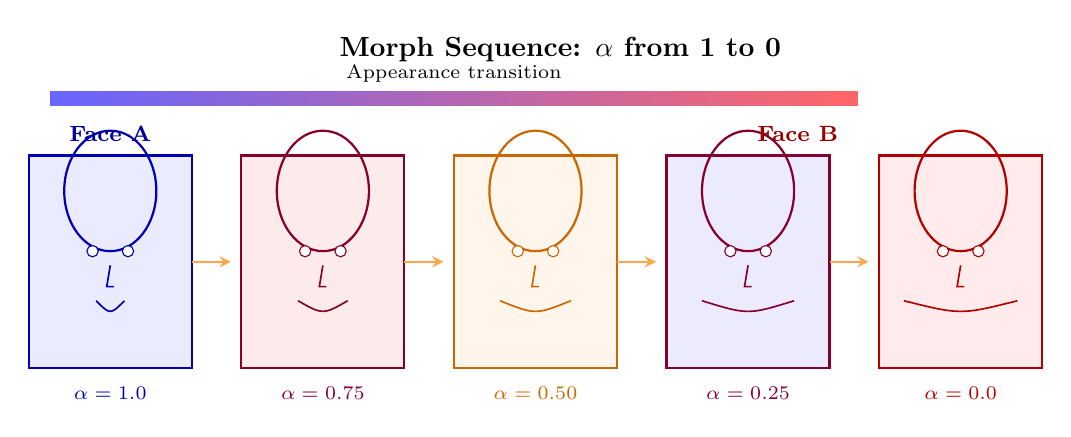
\begin{tikzpicture}[>=stealth, scale=0.9]
    % Title
    \node[font=\normalsize\bfseries] at (7.5, 5.0) {Morph Sequence: $\alpha$ from 1 to 0};

    % Five panels
    \foreach \i/\lbl/\bg/\fg in {%
        0/{$\alpha = 1.0$}/blue!8/blue!70!black,%
        1/{$\alpha = 0.75$}/blue!8!red!8/purple!70!black,%
        2/{$\alpha = 0.50$}/orange!8/orange!80!black,%
        3/{$\alpha = 0.25$}/red!8!blue!8/purple!70!black,%
        4/{$\alpha = 0.0$}/red!8/red!70!black%
    } {
        \pgfmathsetmacro{\xpos}{\i * 3.0}

        % Panel border
        \filldraw[thick, draw=\fg, fill=\bg] (\xpos, 0.5) rectangle (\xpos + 2.3, 3.5);

        % Stylized face outline inside panel
        \begin{scope}[shift={(\xpos + 1.15, 2.0)}]
            % Head shape
            \draw[color=\fg, line width=0.8pt] (0, 1.0) ellipse [x radius=0.65, y radius=0.85];
            % Eyes
            \filldraw[color=\fg, fill=white] (-0.25, 0.15) circle (0.08);
            \filldraw[color=\fg, fill=white] (0.25, 0.15) circle (0.08);
            % Nose
            \draw[color=\fg, line width=0.6pt] (0, -0.05) -- (-0.05, -0.35) -- (0.05, -0.35);
            % Mouth - varies with alpha
            \pgfmathsetmacro{\mouthwidth}{0.2 + 0.15*\i}
            \draw[color=\fg, line width=0.6pt] (-\mouthwidth, -0.55) .. controls (0, -0.75) .. (\mouthwidth, -0.55);
        \end{scope}

        % Alpha label below
        \node[font=\scriptsize, color=\fg] at (\xpos + 1.15, 0.15) {\lbl};

        % Arrows between panels
        \ifnum \i < 4
            \draw[->, thick, orange!70] (\xpos + 2.3, 2.0) -- (\xpos + 2.85, 2.0);
        \fi
    }

    % Gradient bar at top
    \shade[left color=blue!60, right color=red!60] (0.3, 4.2) rectangle (11.7, 4.4);
    \node[font=\scriptsize] at (6.0, 4.65) {Appearance transition};

    % Face labels
    \node[font=\footnotesize\bfseries, blue!60!black] at (1.15, 3.8) {Face~A};
    \node[font=\footnotesize\bfseries, red!60!black] at (10.85, 3.8) {Face~B};
\end{tikzpicture}
\caption{The morph sequence: five key frames showing a smooth transition from Face~A
($\alpha = 1.0$) through intermediate blends to Face~B ($\alpha = 0.0$). The geometry (mean
shape) evolves at each frame via landmark interpolation, and the colors blend via alpha
compositing. The gradient bar illustrates the continuous appearance transition. Connecting
arrows indicate the temporal progression.}
\label{fig:morph-sequence}
\end{figure}

\subsection{Why We Blend in Mean Shape Space}

The order of operations in the face morphing pipeline is not arbitrary. The correct sequence is:

\begin{center}
\fbox{Warp both faces to mean shape} $\;\longrightarrow\;$ \fbox{Blend the warped images}
\end{center}

It is instructive to understand why the reverse order fails.

\subsubsection{The Wrong Order: Blend Then Warp}

Suppose we first blend the \emph{original} (unwarped) Face~A and Face~B, and then attempt to
warp the result to the mean shape:

\begin{center}
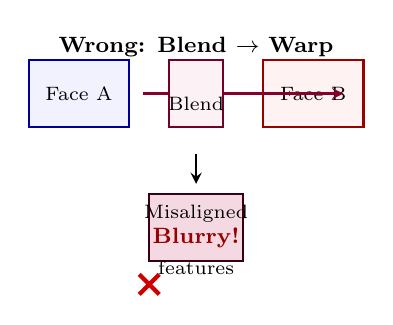
\begin{tikzpicture}[>=stealth, scale=0.85]
    % Top row: wrong order
    \node[font=\bfseries\footnotesize] at (0, 3.2) {Wrong: Blend $\rightarrow$ Warp};

    % Original faces
    \filldraw[thick, draw=blue!60!black, fill=blue!5] (-2.5, 2.0) rectangle (-1.0, 3.0);
    \node[font=\scriptsize, align=center] at (-1.75, 2.5) {Face~A};

    \filldraw[thick, draw=red!60!black, fill=red!5] (1.0, 2.0) rectangle (2.5, 3.0);
    \node[font=\scriptsize, align=center] at (1.75, 2.5) {Face~B};

    % Blend arrow
    \draw[->, thick, purple!70!black] (-0.8, 2.5) -- (-0.1, 2.5);
    \draw[<-, thick, purple!70!black] (0.1, 2.5) -- (0.8, 2.5);

    % Blended (unwarped)
    \filldraw[thick, draw=purple!60!black, fill=purple!5] (-0.4, 2.0) rectangle (0.4, 3.0);
    \node[font=\scriptsize, align=center] at (0, 2.35) {Blend};

    % Warp arrow
    \draw[->, thick, purple!70!black] (0.4, 2.5) -- (2.2, 2.5);
    \draw[->, thick] (0, 1.6) -- (0, 1.15);

    % Result (warped blend)
    \filldraw[thick, draw=purple!30!black, fill=purple!15] (-0.7, 0.0) rectangle (0.7, 1.0);
    \node[font=\footnotesize\bfseries, red!60!black] at (0, 0.35) {Blurry!};
    \node[font=\scriptsize, align=center] at (0, 0.7) {Misaligned};
    \node[font=\scriptsize, align=center] at (0, -0.1) {features};

    % X mark
    \draw[red!80!black, line width=1.5pt] (-0.85, -0.5) -- (-0.55, -0.2);
    \draw[red!80!black, line width=1.5pt] (-0.55, -0.5) -- (-0.85, -0.2);
\end{tikzpicture}
\end{center}

The problem is geometric: Face~A's left eye might be at pixel $(120, 80)$ while Face~B's left
eye is at $(150, 90)$. If we blend first, the resulting pixel at $(120, 80)$ is a mix of
Face~A's eye and Face~B's \emph{cheek} (since Face~B's eye is elsewhere). The blend already
contains a ghosted, misaligned superposition. Warping this blurred result to the mean shape
cannot recover the lost detail --- it merely deforms the blur.

More formally, the pixel-wise blending in Equation~\eqref{eq:alpha-blend-scalar} assumes that
$W_A(x, y)$ and $W_B(x, y)$ represent \emph{corresponding} image content at position $(x, y)$.
When the images are not geometrically aligned, this assumption is violated, and the linear
combination no longer has a meaningful interpretation.

\subsubsection{The Correct Order: Warp Then Blend}

Now consider the correct sequence. First, each face is warped independently to the mean shape:

\begin{center}
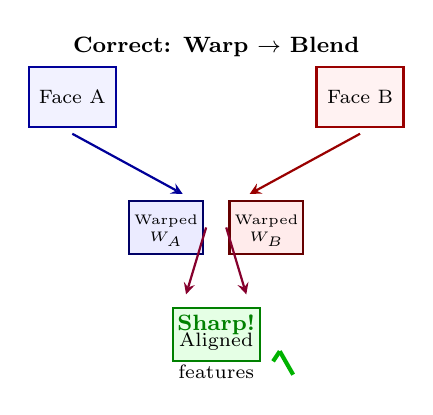
\begin{tikzpicture}[>=stealth, scale=0.85]
    % Bottom row: correct order
    \node[font=\bfseries\footnotesize] at (0, 3.2) {Correct: Warp $\rightarrow$ Blend};

    % Original faces
    \filldraw[thick, draw=blue!60!black, fill=blue!5] (-2.8, 2.0) rectangle (-1.5, 2.9);
    \node[font=\scriptsize, align=center] at (-2.15, 2.45) {Face~A};

    \filldraw[thick, draw=red!60!black, fill=red!5] (1.5, 2.0) rectangle (2.8, 2.9);
    \node[font=\scriptsize, align=center] at (2.15, 2.45) {Face~B};

    % Warp arrows (down and inward)
    \draw[->, thick, blue!60!black] (-2.15, 1.9) -- (-0.5, 1.0);
    \draw[->, thick, red!60!black] (2.15, 1.9) -- (0.5, 1.0);

    % Warped faces in mean shape
    \filldraw[thick, draw=blue!40!black, fill=blue!8] (-1.3, 0.1) rectangle (-0.2, 0.9);
    \node[font=\tiny, align=center] at (-0.75, 0.45) {Warped\\$W_A$};

    \filldraw[thick, draw=red!40!black, fill=red!8] (0.2, 0.1) rectangle (1.3, 0.9);
    \node[font=\tiny, align=center] at (0.75, 0.45) {Warped\\$W_B$};

    % Blend arrows
    \draw[->, thick, purple!70!black] (-0.15, 0.5) -- (-0.45, -0.5);
    \draw[->, thick, purple!70!black] (0.15, 0.5) -- (0.45, -0.5);

    % Blended result
    \filldraw[thick, draw=green!50!black, fill=green!10] (-0.65, -1.5) rectangle (0.65, -0.7);
    \node[font=\footnotesize\bfseries, green!50!black] at (0, -0.95) {Sharp!};
    \node[font=\scriptsize, align=center] at (0, -1.2) {Aligned};
    \node[font=\scriptsize, align=center] at (0, -1.65) {features};

    % Checkmark
    \draw[green!70!black, line width=1.5pt] (0.85, -1.5) -- (0.95, -1.35);
    \draw[green!70!black, line width=1.5pt] (0.95, -1.35) -- (1.15, -1.7);
\end{tikzpicture}
\end{center}

After warping, both $W_A$ and $W_B$ have Face~A's left eye and Face~B's left eye at the
\emph{same} pixel coordinate in the mean-shape canvas. The blending operation now combines
corresponding features with corresponding features. The result is sharp because the input
to the blend is already geometrically registered.

The key insight is that the Delaunay triangulation and piecewise affine warp establish a
``pixel correspondence'' between the two images. Once this correspondence is established,
simple linear blending is sufficient to produce a natural-looking composite.

\subsubsection{Summary of Artifact Comparison}

\begin{table}[htbp]
\centering
\caption{Comparison of blending orders and their visual consequences.}
\label{tab:blend-order}
\begin{tabular}{@{}lcc@{}}
\toprule
& \textbf{Blend $\rightarrow$ Warp} & \textbf{Warp $\rightarrow$ Blend} \\
\midrule
Spatial alignment & No (features at different locations) & Yes (both in mean shape) \\
Feature correspondence & Pixel $p$ in A $\neq$ pixel $p$ in B & Pixel $p$ in A $\approx$ pixel $p$ in B \\
Blending artifacts & Ghosting, blur, doubling & None (assuming good landmarks) \\
Geometric distortion & Warped blur (irreversible) & None \\
Final quality & Poor & Excellent \\
\bottomrule
\end{tabular}
\end{table}

\subsection{Advanced Blending Techniques}

While simple alpha blending produces good results for most face morphing applications, several
advanced techniques can further improve quality in challenging cases.

\subsubsection{Multi-Band (Laplacian Pyramid) Blending}

Multi-band blending decomposes images into frequency bands using a \textbf{Laplacian pyramid}
and blends each band with a different strategy. The intuition is:

\begin{itemize}
    \item \textbf{Low frequencies} (smooth gradients, overall brightness) can be blended with a
          gentle, gradual transition. These carry the overall color and lighting.
    \item \textbf{High frequencies} (edges, fine texture) benefit from a sharper transition to
          avoid blurring or visible seams along triangle boundaries.
\end{itemize}

\paragraph{Pyramid decomposition.} The Laplacian pyramid is constructed as follows:

\begin{enumerate}
    \item Start with the image $I_0 = I$ at full resolution.
    \item \textbf{Gaussian pyramid:} Repeatedly blur and downsample:
          \begin{equation}
              I_{k} = \text{blur}\bigl(\text{downsample}(I_{k-1})\bigr), \qquad k = 1, 2, \ldots, L,
          \end{equation}
          where $L$ is the pyramid depth.
    \item \textbf{Laplacian pyramid:} At each level, compute the difference between the current
          level and the upsampled, blurred version of the next level:
          \begin{equation}
              \mathcal{L}_k = I_k - \text{upsample}\bigl(\text{blur}(I_{k+1})\bigr),
              \qquad k = 0, 1, \ldots, L - 1.
          \end{equation}
          The top level $\mathcal{L}_L = I_L$ is the coarsest Gaussian level.
\end{enumerate}

Each level $\mathcal{L}_k$ captures detail at a specific spatial frequency. The original image
can be perfectly reconstructed by summing all levels:

\begin{equation}
    I = \sum_{k=0}^{L} \mathcal{L}_k.
\end{equation}

For blending, we construct Laplacian pyramids for both $W_A$ and $W_B$, then blend each level
with its own weighting $\alpha_k$. Typically, $\alpha_k$ is more aggressive (closer to a
step function) at high frequencies and more gentle at low frequencies. The final blended image
is reconstructed by collapsing the blended pyramid.

This approach eliminates visible seams that can appear at triangle boundaries, because the
sharp discontinuities are pushed into the highest frequency bands where they are less
perceptible.

\subsubsection{Poisson Blending}

Poisson blending formulates the blending problem as solving a \textbf{Poisson equation} in the
gradient domain. Instead of directly averaging pixel values, it seeks an output image $O$ whose
gradient field best matches a target gradient, subject to boundary conditions:

\begin{equation}
    \Delta O = \nabla \cdot \mathbf{v},
\end{equation}

where $\mathbf{v}$ is the \emph{guidance vector field} (typically the gradient of one of the
input images or a combination), $\Delta$ is the Laplacian operator, and $\nabla \cdot$ is the
divergence.

In the context of face morphing, Poisson blending can be used to seamlessly merge the two
warped images by matching the gradients along triangle boundaries. It is more commonly used
for image compositing (pasting objects into new backgrounds) but can reduce seam artifacts in
morphing when the two faces have significantly different lighting or contrast.

The main drawback is computational cost: solving the Poisson equation requires solving a large
sparse linear system, typically via iterative methods (e.g., multigrid or conjugate gradient).

\subsubsection{Feature-Weighted Blending}

Instead of using a uniform $\alpha$ across the entire image, we can define a
\textbf{spatially-varying blending weight} $\alpha(x, y)$:

\begin{equation}
    O(x, y) = \alpha(x, y) \cdot W_A(x, y) + (1 - \alpha(x, y)) \cdot W_B(x, y).
\end{equation}

The weight function $\alpha(x, y)$ can be designed to emphasize facial regions where identity
is most recognizable:

\begin{itemize}
    \item \textbf{Eyes, nose, mouth:} Give higher weight to the face whose features are clearer
          or more expressive in these regions.
    \item \textbf{Face boundary / hairline:} Transition smoothly to avoid a visible seam where
          the face meets the background.
    \item \textbf{Smoothness:} The weight function itself must be smooth to avoid introducing
          new artifacts. A common choice is a Gaussian-weighted mask centered on each facial
          feature.
\end{itemize}

This technique gives the user fine-grained artistic control, allowing them to, for example,
preserve Face~A's eyes and smile while taking Face~B's jawline and forehead.

\subsubsection{Comparison of Techniques}

\begin{table}[htbp]
\centering
\caption{Comparison of blending techniques.}
\label{tab:blending-comparison}
\begin{tabular}{@{}lcccc@{}}
\toprule
\textbf{Technique} & \textbf{Complexity} & \textbf{Quality} & \textbf{Speed} & \textbf{When to Use} \\
\midrule
Alpha blending & Low & Good & Very fast & Default choice; most cases \\
Multi-band blending & Medium & Very good & Fast & Visible seams; lighting mismatch \\
Poisson blending & High & Excellent & Slow & Significant lighting/contrast differences \\
Feature-weighted & Medium & User-dependent & Fast & Artistic control; selective features \\
\bottomrule
\end{tabular}
\end{table}

For the vast majority of face morphing tasks, simple alpha blending with good landmark
correspondence produces excellent results. The advanced techniques are most valuable when
the input faces differ substantially in lighting, exposure, or background.

\subsection{Post-Processing}

After the blending step, a few optional post-processing operations can polish the final result.

\subsubsection{Color Correction}

If Face~A and Face~B have different overall brightness or color balance, the blended result may
appear slightly off. A simple correction matches the mean and variance of the output to the
inputs:

\begin{equation}
    O_{\text{corrected}}(x, y) = \sigma_{\text{target}}
        \cdot \frac{O(x, y) - \mu_O}{\sigma_O} + \mu_{\text{target}},
\end{equation}

where $\mu_O$ and $\sigma_O$ are the mean and standard deviation of the blended image, and
$\mu_{\text{target}}$, $\sigma_{\text{target}}$ are the desired statistics (e.g., the average
of the two input means). This is a per-channel operation applied independently to R, G, and B.

A simpler approach is to adjust the overall brightness so that the mean intensity of the output
equals the average of the mean intensities of the two warped inputs.

\subsubsection{Boundary Smoothing}

Minor artifacts can persist at Delaunay triangle edges after blending. A mild Gaussian blur
applied to the final result can help:

\begin{equation}
    O_{\text{smooth}}(x, y) = \sum_{u, v} G_\sigma(u, v) \cdot O(x - u, y - v),
\end{equation}

where $G_\sigma$ is a 2D Gaussian kernel with a small standard deviation
($\sigma \approx 0.5$--1.0 pixels). This is subtle enough to avoid noticeable loss of sharpness
while eliminating sub-pixel seams.

In practice:

\begin{minted}{python}
import cv2

# sigma = 0.8 is a gentle default
smoothed = cv2.GaussianBlur(blended, ksize=(3, 3), sigmaX=0.8)
\end{minted}

\subsubsection{Vignetting and Aesthetic Touches}

For presentation-quality output, post-processing may include:

\begin{itemize}
    \item \textbf{Vignetting:} Darken the image edges with a radially symmetric falloff to draw
          attention to the face center. Applied as a per-pixel multiplication:
          \begin{equation}
              O_{\text{vignette}}(x, y) = v(r) \cdot O(x, y), \quad
              r = \frac{\sqrt{(x - c_x)^2 + (y - c_y)^2}}{r_{\text{max}}},
          \end{equation}
          where $v(r)$ decreases from 1 at the center to about 0.7 at the corners.
    \item \textbf{Contrast enhancement:} A slight S-curve in the tone curve can make the result
          pop.
    \item \textbf{Cropping:} Tight crop to the face region removes any black borders or
          background artifacts from the warping step.
\end{itemize}

These steps are optional and depend on the intended use case. For algorithmic evaluation, raw
output without post-processing is preferred. For presentations, a light touch of vignetting
and contrast enhancement goes a long way.
